\documentclass[a4paper, oneside]{memoir}
\usepackage[utf8]{inputenc}
\usepackage[T1]{fontenc}
\usepackage{pifont}
\usepackage{amssymb}
\usepackage{fourier}
\usepackage[dvipsnames]{xcolor}
\usepackage{tikz}
\usepackage{pdfpages}
\usepackage[sfdefault]{roboto}
\usepackage{color}

% Styles
\tikzstyle{teamshare} = [below, text width=5.4cm, inner sep = 0.5cm, text=white, align=center]
\tikzstyle{cardtext} = [below, text width=5.9cm, inner sep = 0.25cm, text centered]
\setlrmarginsandblock{0.9cm}{*}{1}
\setulmarginsandblock{1.49cm}{*}{1}
\checkandfixthelayout[nearest]
\pagestyle{empty}

% Define Commands
\newcommand{\condition}[1]{\textbf{#1}}
\newcommand{\character}[1]{\textbf{#1}}
\newdimen\titlespacing
\titlespacing=0.15cm

% Define Seperators
\newcommand{\seperator}[1]{\\ \vspace{\titlespacing} \hrulefill {} \tiny \bfseries #1 \normalfont \normalsize \hrulefill \\ \vspace{\titlespacing}}
\newcommand{\seperatoraction}{\seperator{POWER}}
\newcommand{\seperatordescription}{\seperator{DESCRIPTION}}
\newcommand{\seperatorcondition}{\seperator{CONDITION}}
\newcommand{\seperatorwin}{\seperator{HOW TO WIN}}
\newcommand{\redwinsection}{
	\seperatorwin
	\small You win if \character{President} gains the \condition{dead} condition due to the \character{Bomber} exploading.
}
\newcommand{\bluewinsection}{
	\seperatorwin
	\small You win if \character{President} does not gain the \condition{dead} condition due to the \character{Bomber} exploading.
}
\newcommand{\titlefrom}[1]{\\ \tiny > from #1 <\normalsize}

% Begin Document
\begin{document}
	
	% New Page
	\noindent 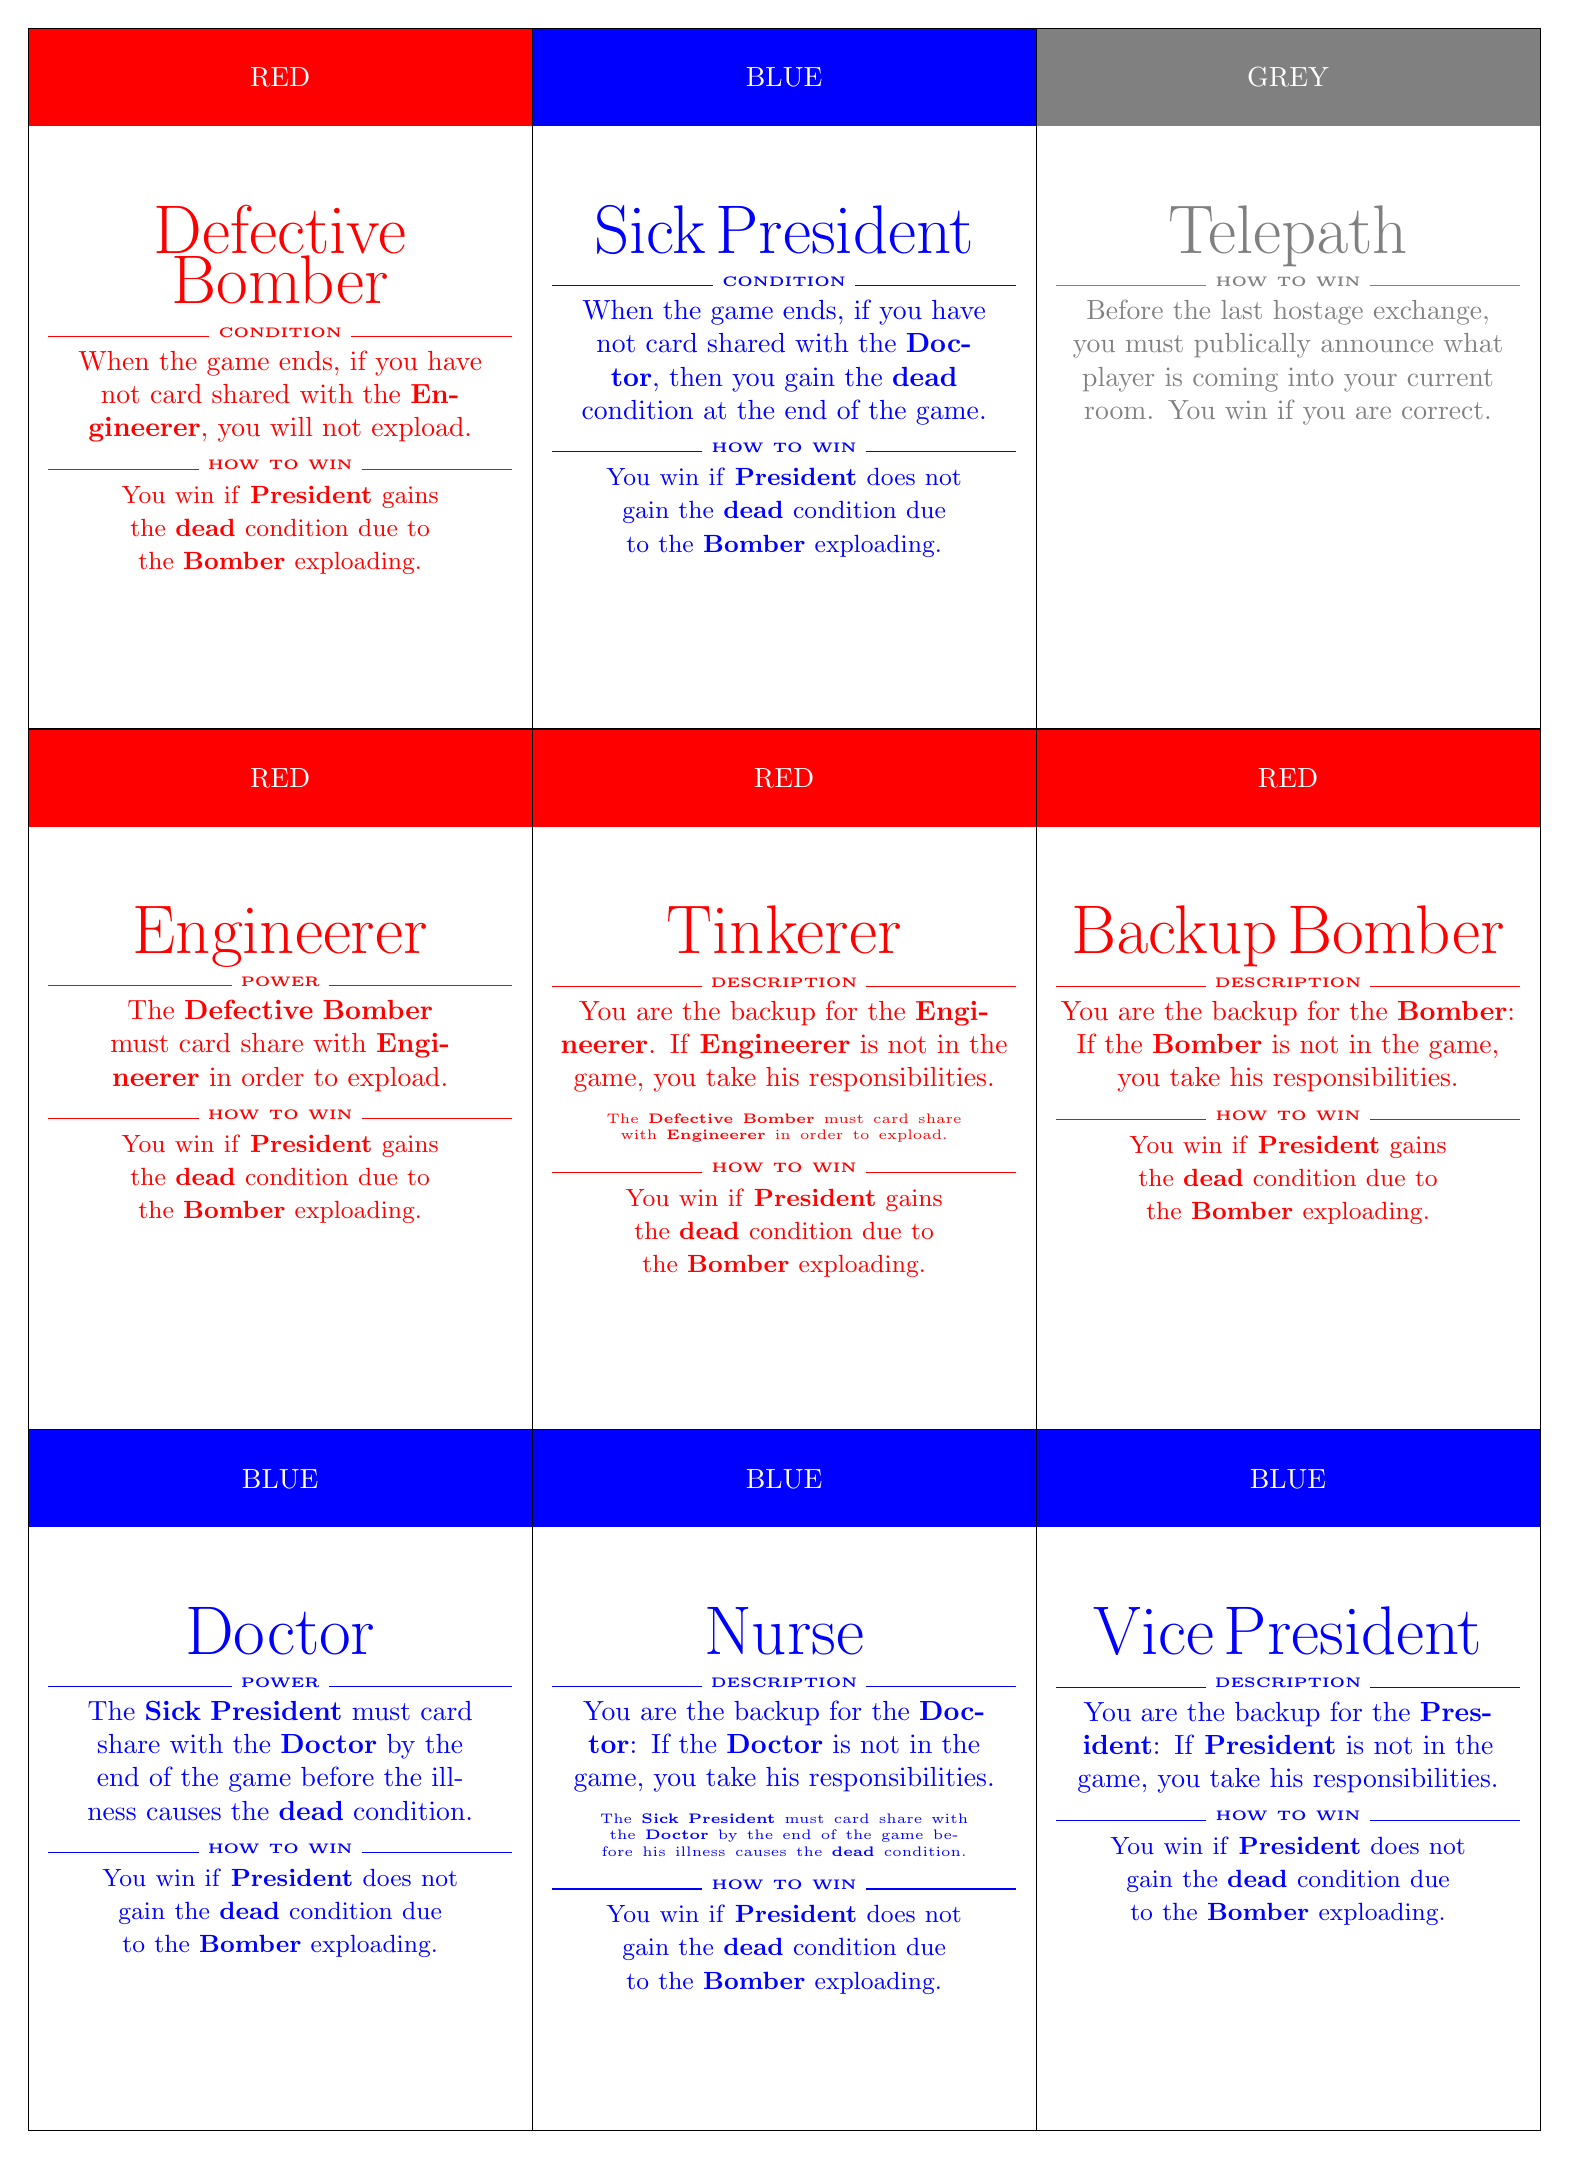
\begin{tikzpicture}[outer sep=0]

% DEFECTIVE BOMBER
\node[teamshare, fill=red] (1) at (3.2,26.7) {\HUGE RED};
\node[cardtext, text=red] at (3.2,24.7) {
	{\Huge Defective Bomber}
	\seperatorcondition
	When the game ends, if you have not card shared with the \character{Engineerer}, you will not expload.
	\redwinsection
};

% SICK PRESIDENT
\node[teamshare, fill=blue] at (9.6,26.7) {\HUGE BLUE};
\node[cardtext, text=blue] at (9.6,24.7) {
	{\Huge Sick President}
	\seperatorcondition
	When the game ends, if you have not card shared with the \character{Doctor}, then you gain the \condition{dead} \\ condition at the end of the game.
	\bluewinsection
};

% TELEPATH
\node[teamshare, fill=gray] at (16,26.7) {\HUGE GREY};
\node[cardtext, text=gray] at (16,24.7) {
	{\Huge Telepath}
	\seperatorwin
	Before the last hostage exchange, you must publically announce what player is coming into your current room. You win if you are correct.
};

% ENGINEERER
\node[teamshare, fill=red] at (3.2,17.8) {\HUGE RED};
\node[cardtext, text=red] at (3.2,15.8) {
	{\Huge Engineerer}
	\seperatoraction
	The \character{Defective Bomber} must card share with \character{Engineerer} in order to expload.
	\redwinsection
};

% TINKERER
\node[teamshare, fill=red] at (9.6,17.8) {\HUGE RED};
\node[cardtext, text=red] at (9.6,15.8) {
	{\Huge Tinkerer}
	\seperatordescription
	You are the backup for the \character{Engineerer}. If \character{Engineerer} is not in the game, you take his responsibilities.
	\\\vspace{0.25cm}
	\tiny The \character{Defective Bomber} must card share with \character{Engineerer} in order to expload.
	\redwinsection
};

% BACKUP BOMBER
\node[teamshare, fill=red] at (16,17.8) {\HUGE RED};
\node[cardtext, text=red] at (16,15.8) {
	{\Huge Backup Bomber}
	\seperatordescription
	You are the backup for the \character{Bomber}: If the \character{Bomber} is not in the game, you take his responsibilities.
	\redwinsection
};

% DOCTOR
\node[teamshare, fill=blue] at (3.2,8.9) {\HUGE BLUE};
\node[cardtext, text=blue] at (3.2,6.9) {
	{\Huge Doctor}
	\seperatoraction
	The \character{Sick President} must card share with the \character{Doctor} by the end of the game before the illness causes the \condition{dead} condition.
	\bluewinsection
};

% NURSE
\node[teamshare, fill=blue] at (9.6,8.9) {\HUGE BLUE};
\node[cardtext, text=blue] at (9.6,6.9) {
	{\Huge Nurse}
	\seperatordescription
	You are the backup for the \character{Doctor}: If the \character{Doctor} is not in the game, you take his responsibilities.
	\\\vspace{0.25cm}
	\tiny The \character{Sick President} must card share with the \character{Doctor} by the end of the game before his illness causes the \condition{dead} condition.
	\bluewinsection
};

% VICE PRESIDENT
\node[teamshare, fill=blue] at (16,8.9) {\HUGE BLUE};
\node[cardtext, text=blue] at (16,6.9) {
	{\Huge Vice President}
	\seperatordescription
	You are the backup for the \character{President}: If \character{President} is not in the game, you take his responsibilities.
	\bluewinsection
};

\draw (0,0) -- (19.2,0);
\draw (0,8.9) -- (19.2,8.9);
\draw (0,17.8) -- (19.2,17.8);
\draw (0,26.7) -- (19.2,26.7);

\draw (0,0) -- (0,26.7);
\draw (6.4,0) -- (6.4,26.7);
\draw (12.8,0) -- (12.8,26.7);
\draw (19.2,0) -- (19.2,26.7);



\end{tikzpicture}

%Background is not my own. But courtesy of a user on BGG
\includepdf[pages={1}, angle=90]{cardsbackground.pdf}

\end{document}